\section{Regulatory compliance}

The present section presents the regulations the proyect complies with. These pertain both to the robot as a whole as to the different third-party components included.

	\subsection{Domestic robots regulations} The project here presented is intended to be used as an assitive domestic robot. This class of robots follow the standard ISO 13482:2014, from 2014-02-19, and which can be found here. \footnote{https://www.iso.org/obp/ui/\#iso:std:iso:13482:ed-1:v1:en}

	\subsection{MJPG-streamer} The video streaming program MJPG-streamer is released under the \textit{GNU General Public License version 2.0 (GPLv2)}. The whole text can be found at \footnote{http://www.gnu.org/licenses/gpl-2.0.html}

	\subsection{Hostapd} This software is licensed under the BSD agreement, which can be found in this website \footnote{http://w1.fi/cgit/hostap/plain/hostapd/README}

	\subsection{Isc-dhcp-server} The Internet Systems Consortium's DHCP server software ir released under the ISC license, similar to the BSD. The whole text can be found here \footnote{http://www.isc.org/downloads/software-support-policy/isc-license/}

	\subsection{Gripper model} The gripper model  used is released under the \textit{Public Domain} license \footnote{http://creativecommons.org/licenses/publicdomain/}, which grants the work to be\textit{freely reproduced, distributed, transmitted, used, modified, built upon, or otherwise exploited by anyone for any purpose, commercial or non-commercial, and in any way, including by methods that have not yet been invented or conceived.}

	\subsection{PD-SD}The Personal Domestic Service Droid is released under the Creative Commons Attribution 4.0 International License \footnote{https://creativecommons.org/licenses/by/4.0/} (Figure \ref{ccby}). This license specifies that \textit{You must give appropriate credit, provide a link to the license, and indicate if changes were made.}\\


	    \begin{figure}[H]
			\centering
	      	
\includegraphics[scale=0.2]{images/ccby}  
	      	\caption{Creative Commons Attribution logo }
			\label{ccby}
		\end{figure}
		









\newpage
\section{Project planning} \label{app:gantt}

This appendix breaks down the project into its different phases and their durations. The project started on 1st November 2013 and finished on the 7th October 2014, with blank periods during January, May and June, due to the examination sessions in the University.  \\

Figure \ref{Ganttresumen} summarizes the phases in a table detailing the duration of each one.
 

	\begin{figure}[H]
	\centering
   	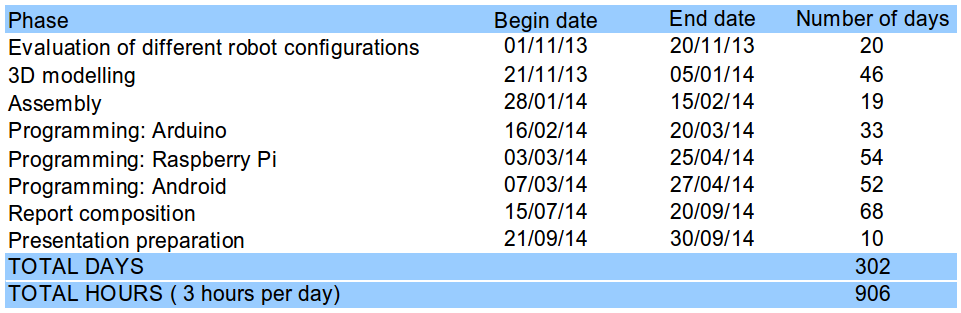
\includegraphics[width=15.5cm]{appendices/Planificacion-Resumen.png} 
   	\caption{Duration of each phase of the project }
	\label{Ganttresumen}
	\end{figure}	


\bigskip

The Gantt diagram corresponding to this planning is shown in Figure \ref{Gantt} 

	\newpage
	\begin{figure}[H]
	\centering
   	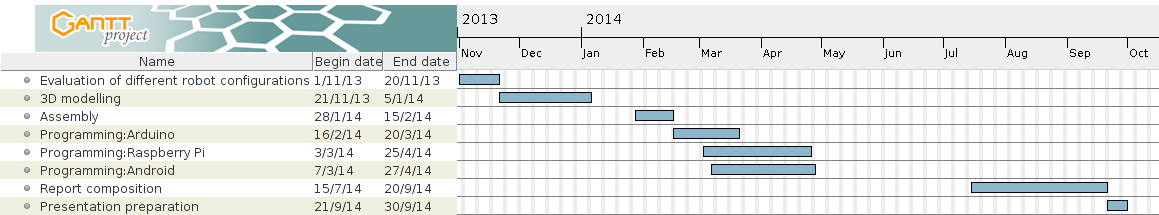
\includegraphics[width=22cm, angle=90]{appendices/Planificacion.png} 
   	\caption{Gantt diagram specifying the duration of each of the project's objectives}
	\label{Gantt}
	\end{figure}





\newpage
\section{Budget} \label{app:bom}

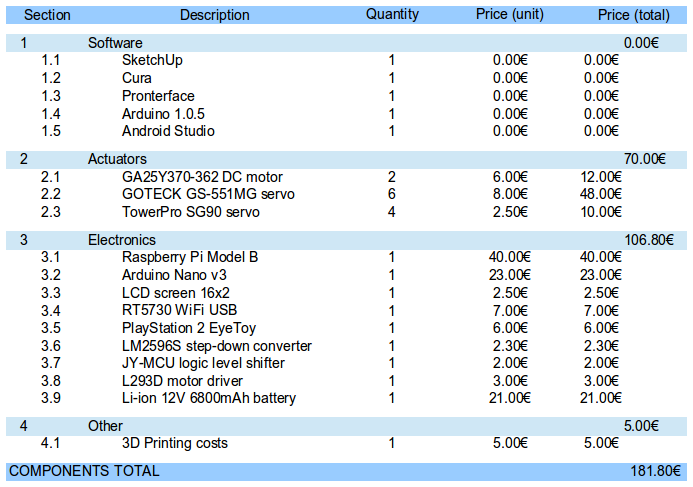
\includegraphics[width=16cm]{appendices/Presupuesto.png}
\bigskip


The robot's components cost is of 181.80 \euro. \\

However, this only takes into account the cost of replicating the robot, not the actual cost of developping the project. In order to get the total cost for this project the engineer's man hours cost must be included, and these can be seen in the previous appendix. \\

The total number of hours being 906 at an hourly rate of 8\euro, the cost of man hours is 906 · 8=7248\euro.\\

Therefore, the project's total cost is 181.80+7248=7429.80\euro.